\documentclass[light]{Theme/lutbeamer} % change between light and dark for the background
%\documentclass[t]{lutbeamer} % use "t" option for top alignment 

\usepackage{pgfpages}
\setbeameroption{hide notes} % Only slides
% \setbeameroption{show only notes} % Only notes
% \setbeameroption{show notes on second screen=right} % Both


\setdepartment{LUT School}
\institute[LUT University]{Lappeenranta–Lahti University of Technology LUT}
\author{Author}
\title[Short presentation title]{Presentation title}
\subtitle{Presentation subtitle}
\date{\today}


\begin{document}

% front page
{ % all template changes are local to this group.
    \setbeamertemplate{navigation symbols}{}
    \begin{frame}<article:0>[plain,noframenumbering]
        \begin{tikzpicture}[remember picture,overlay]
            \node[at=(current page.center)] {
                \includegraphics[
                                 width=\paperwidth,
                                 height=\paperheight]{logos/red_bird.png}
            };
        \end{tikzpicture}
    \end{frame}
}

% Outline
\AtBeginSection[]
{
\begin{frame}[plain,noframenumbering]
\frametitle{Outline}
\begin{columns}[T]
    \begin{column}{0.01\textwidth}
        
    \end{column}
    \begin{column}{0.95\textwidth}
        \tableofcontents[currentsection,
                        %currentsubsection,
                        %hideothersubsections, 
                        %sectionstyle=show/shaded, 
                        %subsectionstyle=show/shaded%/hide
                 ]
    \end{column}
\end{columns}
\end{frame}
}


% use blurred background figure
% {\usebackgroundtemplate{%
% \begin{tikzpicture}[remember picture,overlay]
% \node [anchor=south east, 
%       xshift=2.15cm, 
%       yshift=0.25cm,
%       opacity=0.35, scale=0.3]  at (current page.south east)  {\includegraphics{figures/figurename}};
% \end{tikzpicture}
% }
{ % title page
\begin{frame}[plain]
\maketitle
\small
\par\vskip0.5em
{\footnotesize
    \hspace*{0.2cm}
    \begin{tabular}[t]{@{}l@{\hspace{3pt}}p{.5\textwidth}@{}}
    Supervisor: & Prof. Supervisor, University
    \end{tabular}%
    \par\vskip0.5em
    \hspace*{0.26cm}\begin{tabular}[t]{@{}l@{\hspace{3pt}}p{.5\textwidth}@{}}
    Opponent: & Prof. Opponent, University
    \end{tabular}%
    }
\note[item]{
Honored custos, honored opponent, honored listeners, ...
}
\end{frame}
}

\section{Introduction}
\subsection{Why beamer?}
\begin{frame}
\frametitle{Beamer for LUT slides}
\framesubtitle{}
\begin{itemize}
\item We assume you can use \LaTeX; if you cannot,
\hrefcol{http://en.wikibooks.org/wiki/LaTeX/}{you can learn it here}
\item Beamer is one of the most popular and powerful document classes for presentations in \LaTeX
\item Beamer has also a detailed
\hrefcol{http://www.ctan.org/tex-archive/macros/latex/contrib/beamer/doc/beameruserguide.pdf}{user manual}
\item Here we will present only the most basic features to get you up to speed
\end{itemize}
\end{frame}

\begin{frame}
\frametitle{Beamer vs. PowerPoint}
Compared to PowerPoint, using \LaTeX\ is better because:
\begin{itemize}
\item It is not What-You-See-Is-What-You-Get, but
What-You-\emph{Mean}-Is-What-You-Get:\\
you write the content, the computer does the typesetting
\item Produces a \texttt{pdf}: no problems with fonts, formulas,
      program versions
\item Easier to keep consistent style, fonts, highlighting, etc.
\item Produces side notes
\item Math typesetting in \TeX\ is the best:
\begin{equation*}
\mathrm{i}\,\hslash\frac{\partial}{\partial t} \Psi(\mathbf{r},t) =
-\frac{\hslash^2}{2\,m}\nabla^2\Psi(\mathbf{r},t)
+ V(\mathbf{r})\Psi(\mathbf{r},t)
\end{equation*}

\end{itemize}
\end{frame}

\begin{frame}[fragile]
\frametitle{Selecting the Class}
To start working with \texttt{lutbeamer}, start a \LaTeX\ document with the
preamble:
\begin{block}{Minimum LUT Beamer Document}
\verb|\documentclass[light]{lutbeamer} % or [dark]|\\
\verb|\setbeameroption{hide notes} % or {show only notes} or| 
\verb|% {show notes on second screen=right}|\\
\verb|\begin{document}|\\
\verb|\begin{frame}{Hello, world!}|\\
\verb|\framesubtitle{Subtitle}|\\
\verb|\end{frame}|\\
\verb|\end{document}|\\
\end{block}
\end{frame}

\begin{frame}[fragile]
\frametitle{Title page}
To set a typical title page, you call some commands in the preamble:
\begin{block}{The Commands for the Title Page}
\begin{verbatim}
\setdepartment{LUT School of ... }
\author{Author}
\title[Short presentation title]{Presentation title}
\subtitle{Presentation subtitle}
\date{Defaults to today's}
\end{verbatim}
\end{block}
\end{frame}

\subsection{Writing a Simple Slide}

\begin{frame}[fragile]
\frametitle{Writing a Simple Slide}
\framesubtitle{It's really easy!}
\begin{itemize}[<+->]
\item A typical slide has bulleted lists
\item These can be uncovered in sequence
\end{itemize}
\begin{block}{Code for a Page with an Itemised List}<+->
\begin{verbatim}
\begin{frame}
  \frametitle{Writing a Simple Slide}
  \framesubtitle{It's really easy!}
  \begin{itemize}[<+->]
    \item A typical slide has bulleted lists
    \item These can be uncovered in sequence
  \end{itemize}
\end{frame}\end{verbatim}
\end{block}
\end{frame}

\begin{frame}[fragile]
\frametitle{Using Colours}
\begin{itemize}[<alert@2>]
  \item You can use colours with the
        \verb|\textcolor{<color name>}{text}| command
  \item The colours are defined in the \texttt{lutcolor} package:
  \begin{itemize}
  \item Primary colour: \testcolor{darkblue};
  \item Contrast colours: \testcolor{orange}, \testcolor{black}, \testcolor{pink};
  \item Additional colours: \testcolor{grey}, \testcolor{gr}, 
                            \testcolor{viridian}, \testcolor{rdbu7}
  \end{itemize}
  \item Do \emph{not} abuse colours: \verb|\emph{}| is usually enough
  \item Use \verb|\alert{}| to bring the \alert<2->{focus} somewhere
  \item<2- | alert@2> If you highlight too much, you don't highlight at all!
\end{itemize}
\end{frame}

\begin{frame}[fragile]
\frametitle{Adding images}
\begin{columns}
\begin{column}{0.7\textwidth}
Adding images works like in normal \LaTeX:
\begin{block}{Code for Adding Images}
\begin{verbatim}
\usepackage{graphicx}
% ...
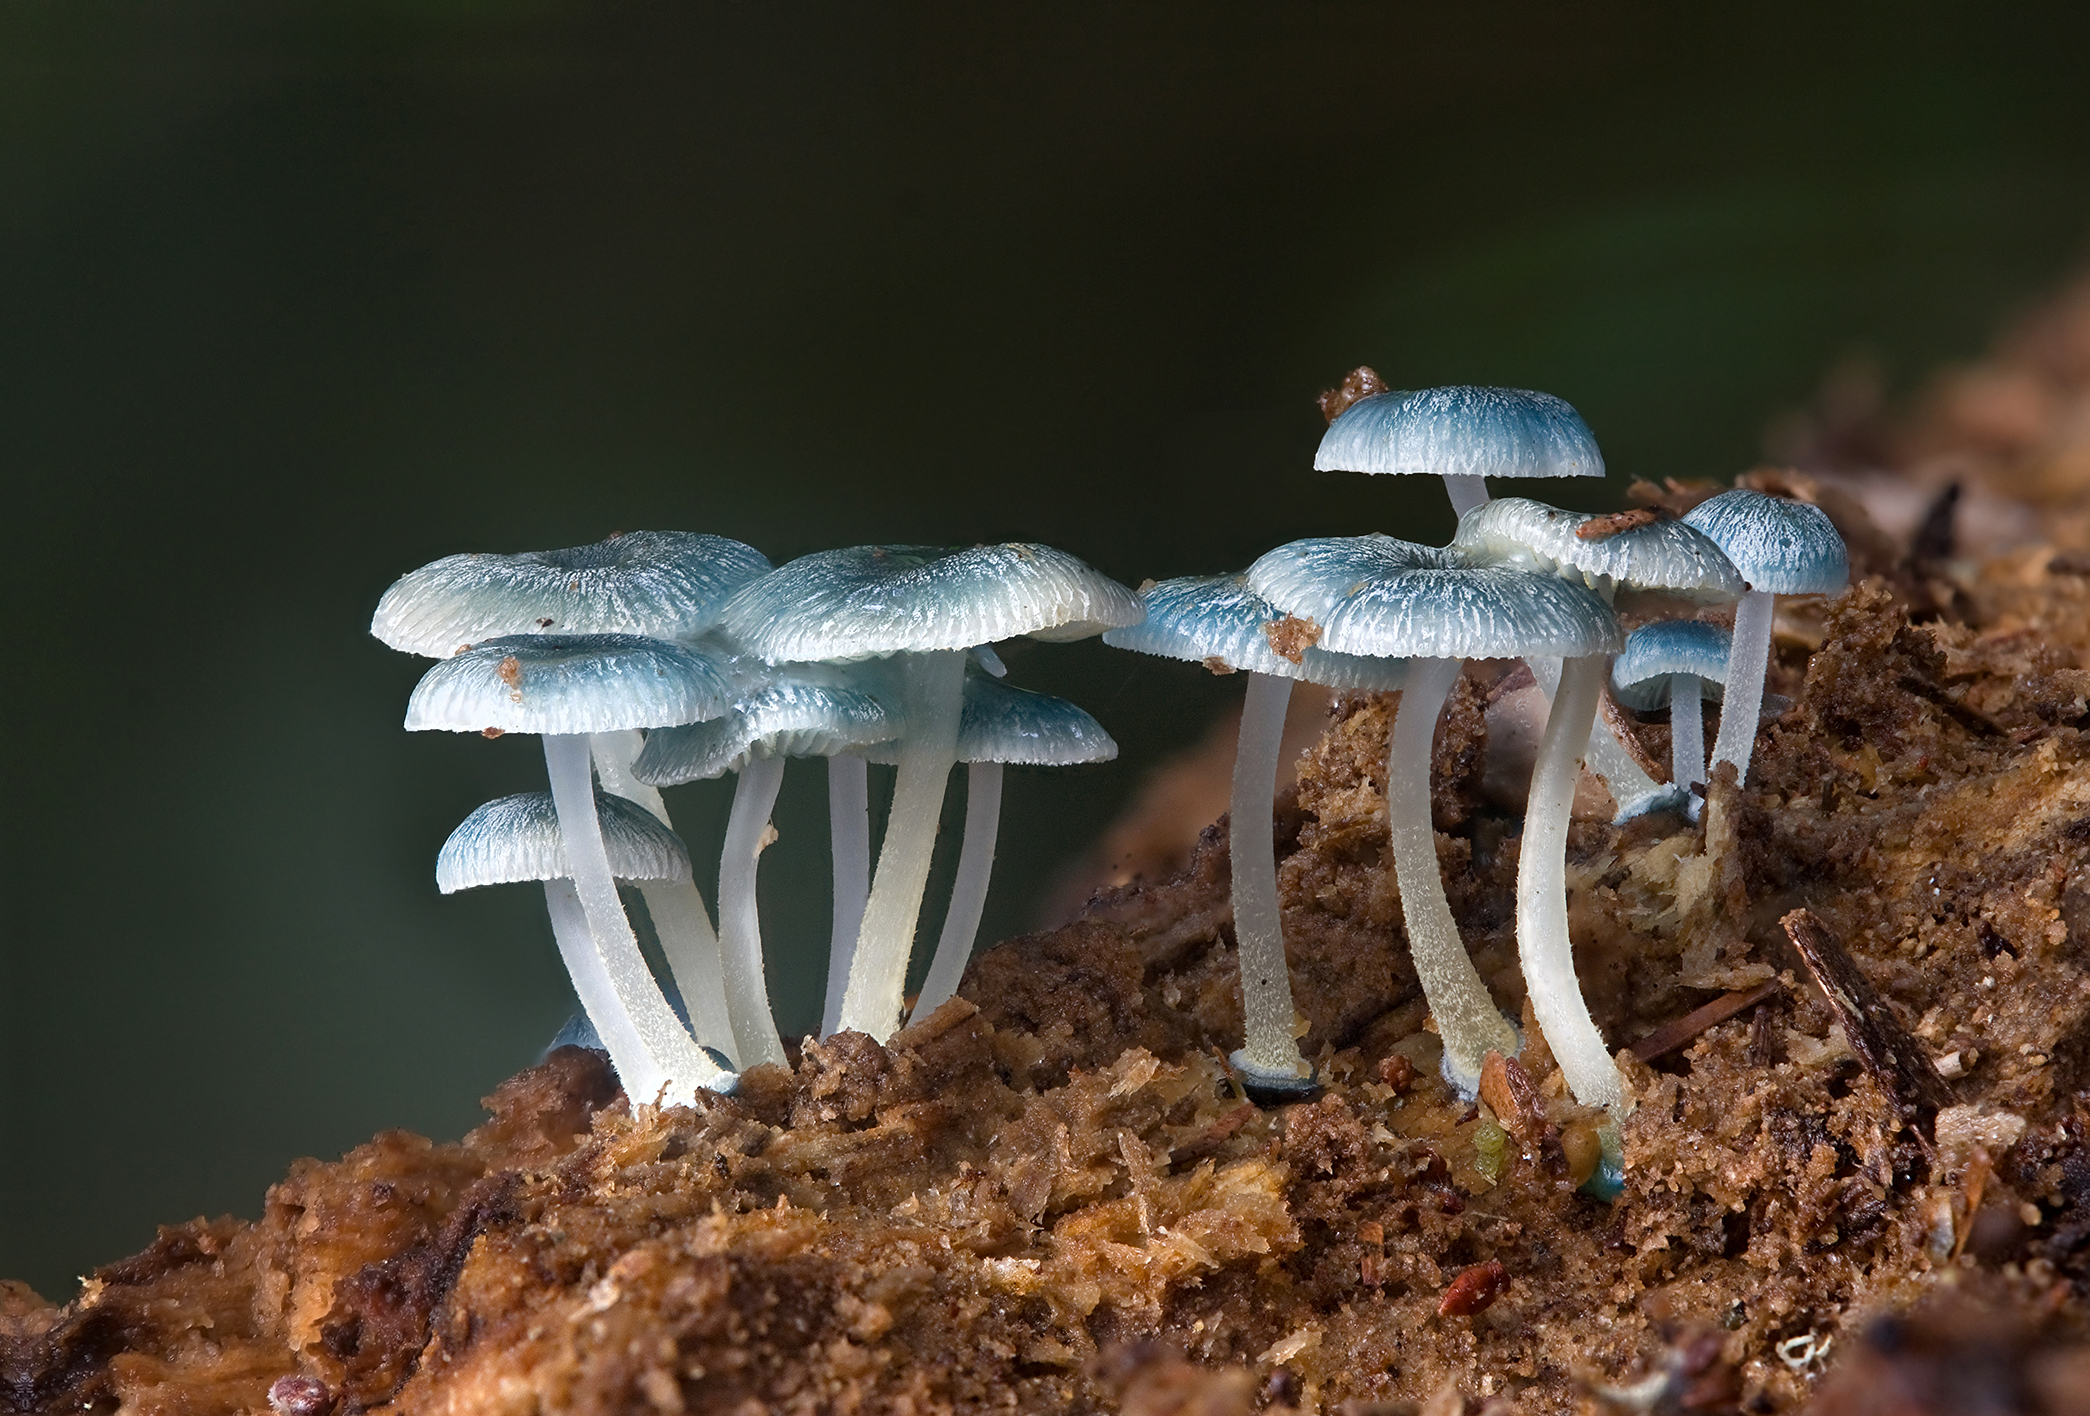
\includegraphics
[width=\textwidth]{figures/Mycena_interrupta}
\end{verbatim}
\end{block}
\end{column}
\begin{column}{0.3\textwidth}
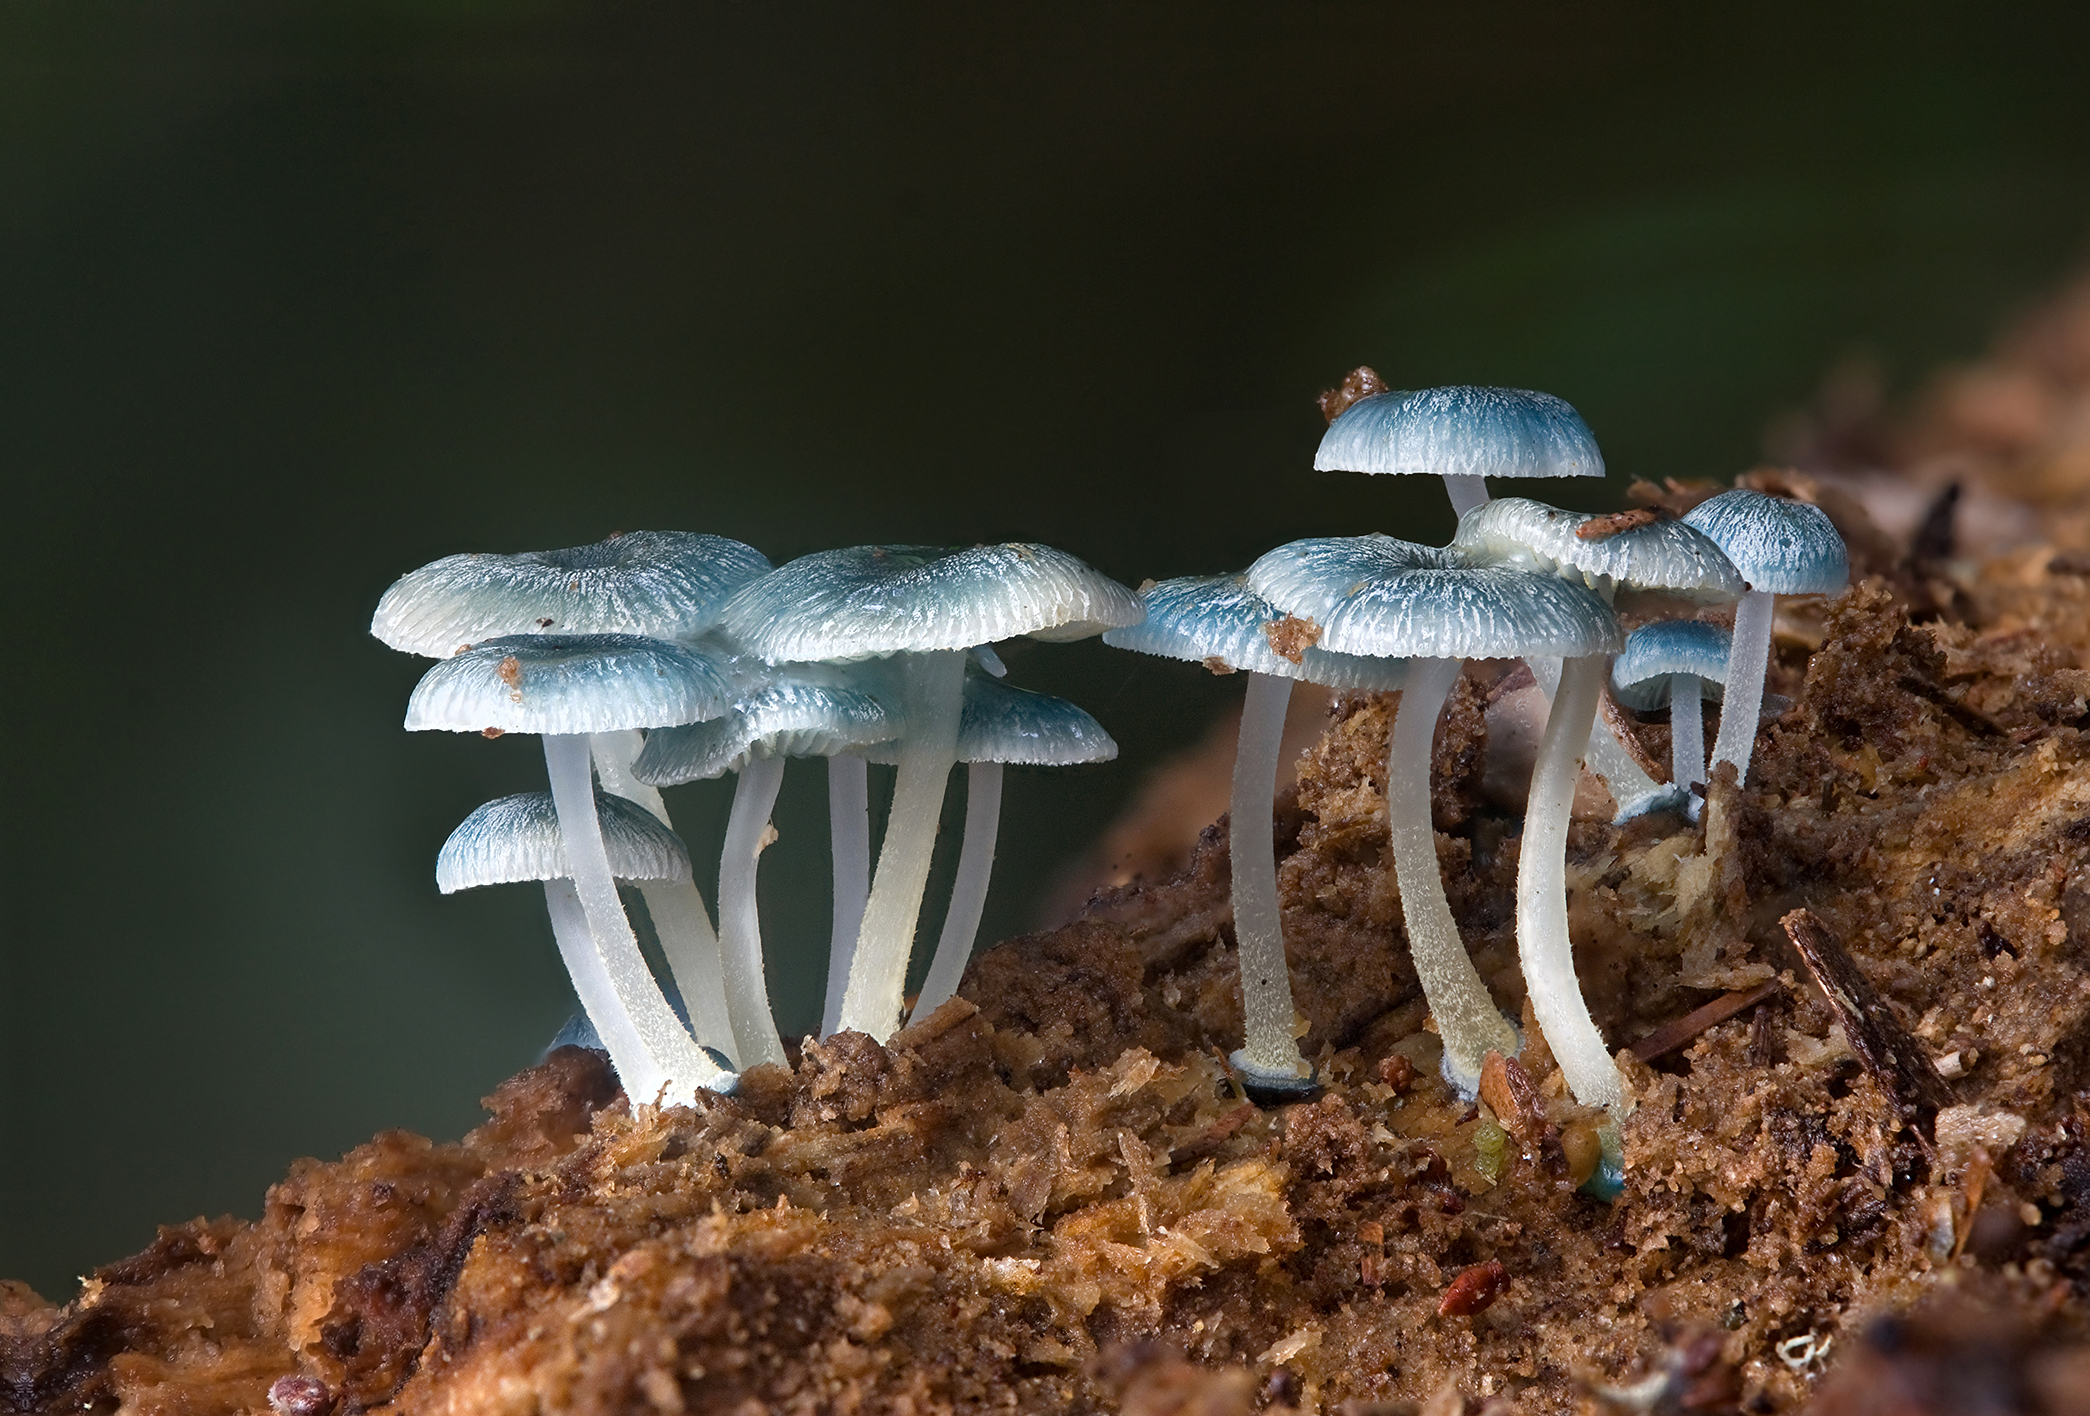
\includegraphics
[width=\textwidth]{figures/Mycena_interrupta}\\
\end{column}
\end{columns}
\end{frame}


\begin{frame}[fragile]
\frametitle{Highlighting an Image region}
\begin{center}
\begin{tikzpicture}
    \node[anchor=south west,inner sep=0] (image) at (0,0) {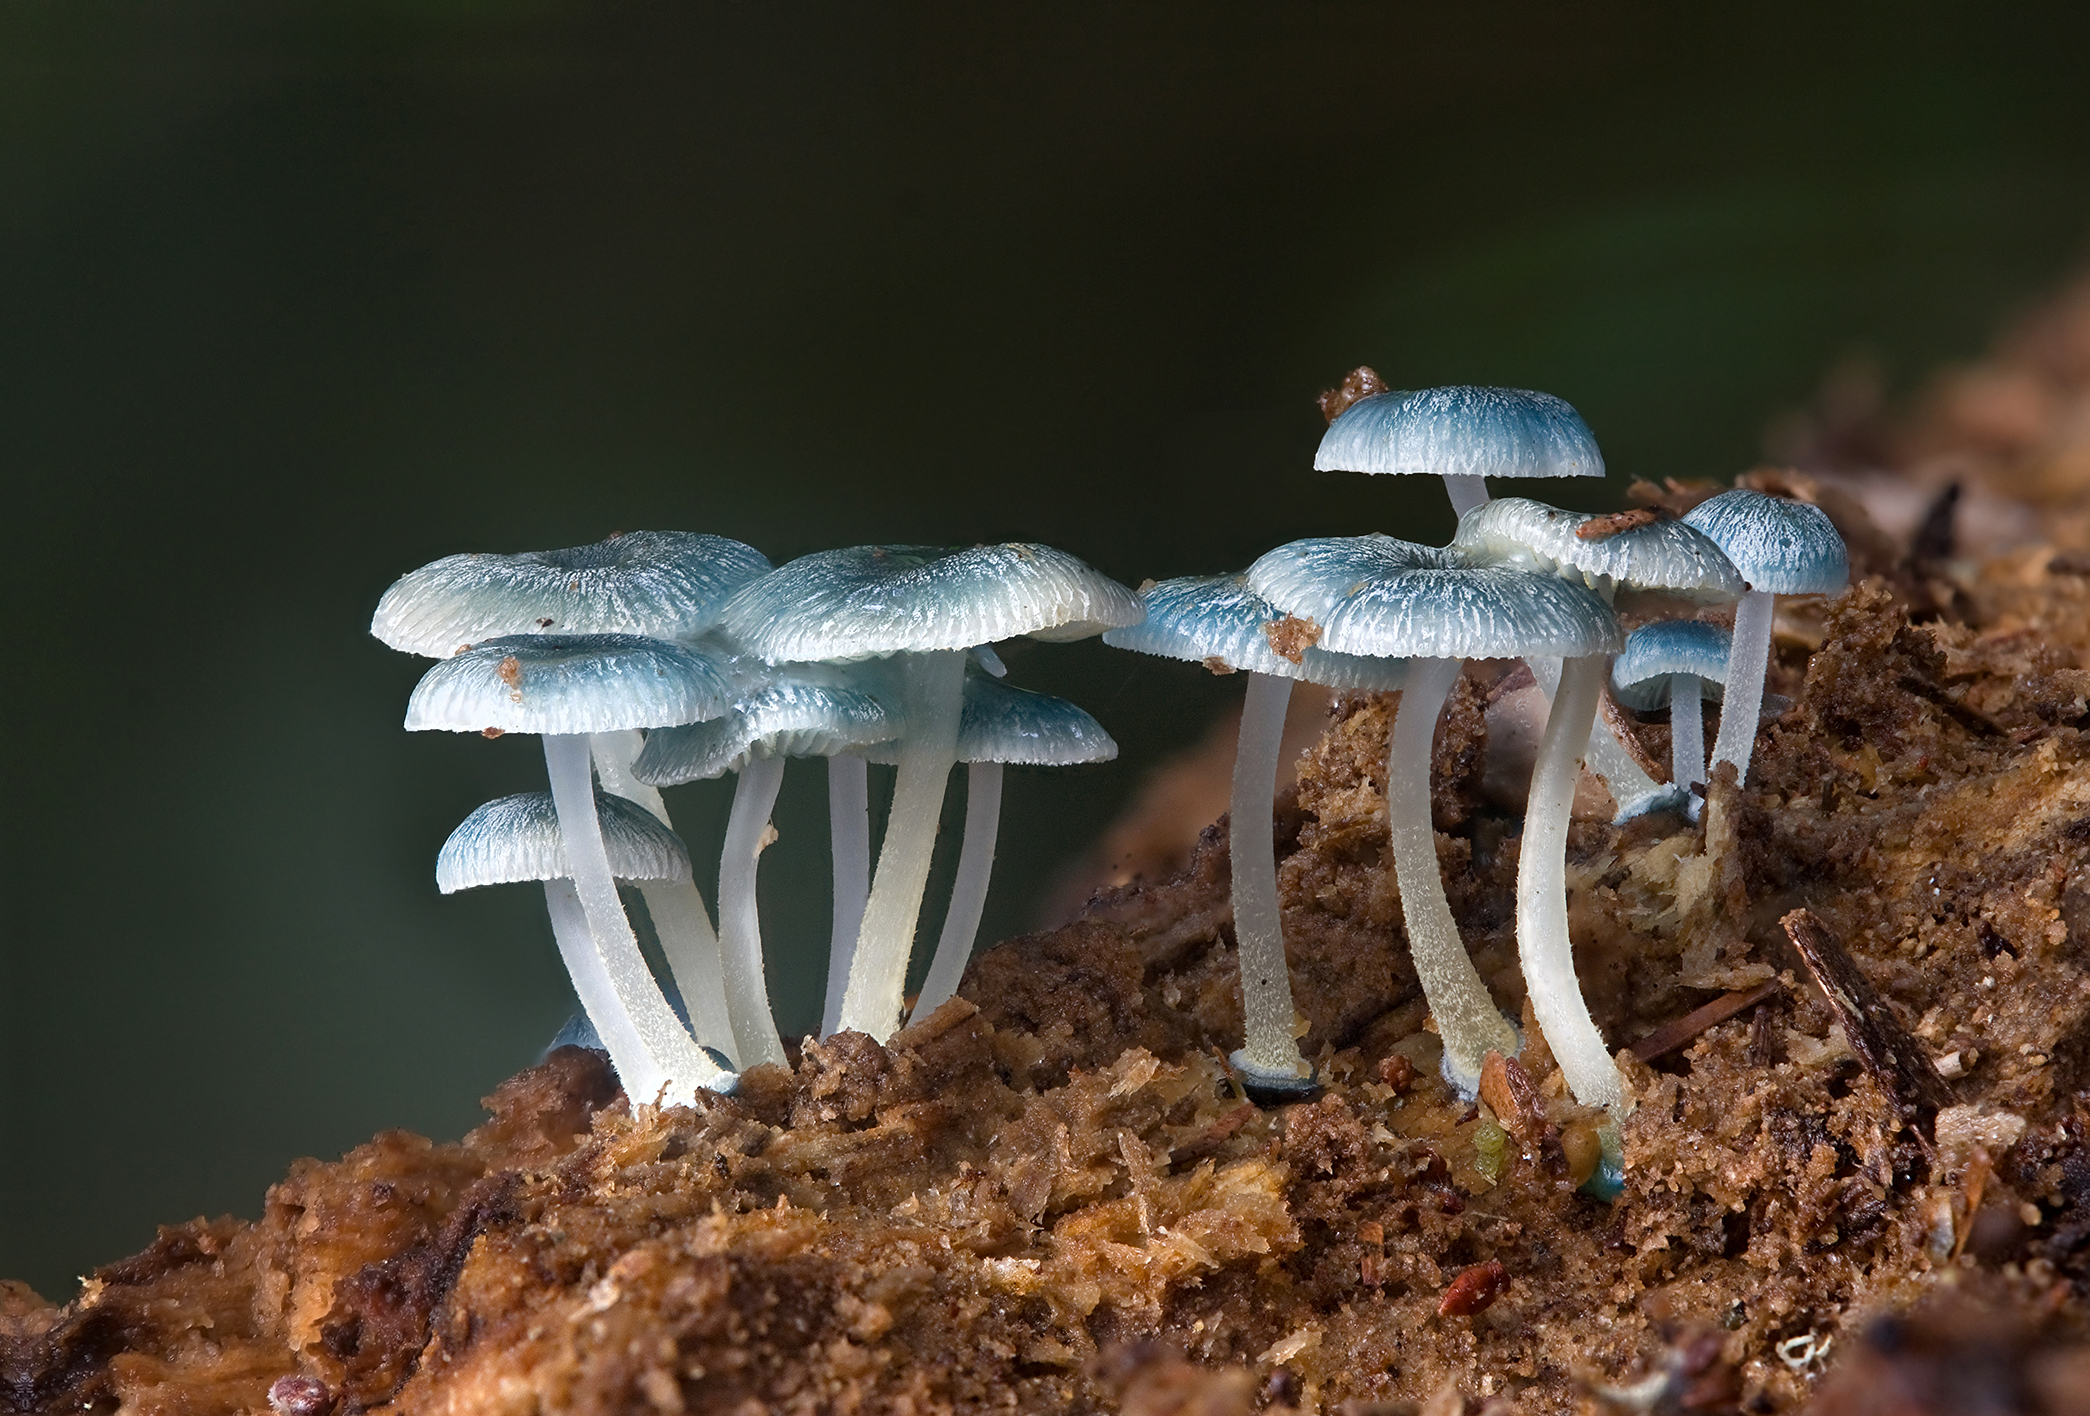
\includegraphics[width=0.6\textwidth]{figures/Mycena_interrupta.jpg}};
    \begin{scope}[x={(image.south east)},y={(image.north west)}]
        \draw[help lines,xstep=.1,ystep=.1] (0,0) grid (1,1);
        \foreach \x in {0,1,...,9} { \node [anchor=north] at (\x/10,0) {0.\x}; }
        \foreach \y in {0,1,...,9} { \node [anchor=east] at (0,\y/10) {0.\y}; }
        \draw[red,ultra thick,rounded corners] (0.6,0.6) rectangle (0.8,0.8);
    \end{scope}
\end{tikzpicture}
\end{center}
\end{frame}

\begin{frame}[fragile]
\frametitle{Splitting in Columns}
Splitting the page is easy and common;
typically, one side has a picture and the other text:
\begin{columns}
\begin{column}{0.6\textwidth}
This is the first column
\end{column}
\begin{column}{0.3\textwidth}
And this the second
\end{column}
\end{columns}
\begin{block}{Column Code}
\begin{verbatim}
\begin{columns}
    \begin{column}{0.6\textwidth}
        This is the first column
    \end{column}
    \begin{column}{0.3\textwidth}
        And this the second
    \end{column}
    % There could be more!
\end{columns}
\end{verbatim}
\end{block}
\end{frame}

\begin{frame}[fragile]
\frametitle{Fonts}
\begin{itemize}
\item The paramount task of fonts is being readable
\item There are good ones...
  \begin{itemize}
  \item {\textrm{Use serif fonts only with high-definition projectors}}
  \item {\textsf{Use sans-serif fonts otherwise (or if you simply prefer them)}}
  \end{itemize}
\item ... and not so good ones:
  \begin{itemize}
  \item {\texttt{Never use monospace for normal text}}
  \item {\frakfamily Gothic, calligraphic or weird fonts: should always: be
  avoided}
\end{itemize}
\end{itemize}
\end{frame}

\begin{frame}[fragile]
\frametitle{Using abbreviations}
To use abbreviations, add new glossary entry in \texttt{nomenclature.tex} file. 
\begin{itemize}
    \item To refer to the entry, use
        \begin{itemize}
            \item \gls{ev}
            \item \Gls{ev}
            \item \glspl{ev}
            \item \glsfirst{ev}
        \end{itemize}
    \end{itemize}

\begin{block}{The Commands for the nomenclature}
\begin{verbatim}
    % ....
        \gls{ev}, \Gls{ev}, \glspl{ev},  \glsfirst{ev}
    % ....     
    \end{verbatim}
\end{block}
\end{frame}


\begin{frame}[fragile]
\frametitle{Look}
\begin{itemize}
\item To change the colour of the title dash, give one of the class options
      \texttt{darkblue} (default), \texttt{orange}, \texttt{pink},
      \texttt{black}, or \texttt{nodash}.
\item To change between the light and dark themes, give the class options
      \texttt{light} (default) or \texttt{dark}. It is not possible to switch
      theme for one slide because of the design of Beamer---and it's probably a
      good thing.
\item The aspect ratio defaults to 16:9, but you can change it to 4:3 for old
      projectors by passing the class option \texttt{aspectratio=43}; any other
      values accepted by Beamer are also possible.
\end{itemize}
\end{frame}


\section{Conclusion}
\subsection{Good luck!}

\begin{frame}
\frametitle{Good Luck!}
\begin{itemize}
\item Enough for an introduction! You should know enough by now
\item If you have corrections or suggestions,
\hrefcol{mailto:mashlakov@gmail.com}{send them to me!}
\end{itemize}
\end{frame}


\appendix % to start a separate page numbering

\begin{frame}
\frametitle{Back-up slides}
\begin{itemize}
    \item You can have some additional info hidden from the main presentation below
\end{itemize}
\end{frame}


\section*{Bibliography}
\begin{frame}[fragile]{Bibliography}
Use BibTeX. Put your bibliography in a separate file (e.g. references.bib): 
In \cite{lamport86} a detailed description of the use of \LaTeX is given.

\printbibliography
\end{frame}


{ % all template changes are local to this group.
    \setbeamertemplate{navigation symbols}{}
    \begin{frame}<article:0>[plain,noframenumbering]
        \begin{tikzpicture}[remember picture,overlay]
            \node[at=(current page.center)] {
                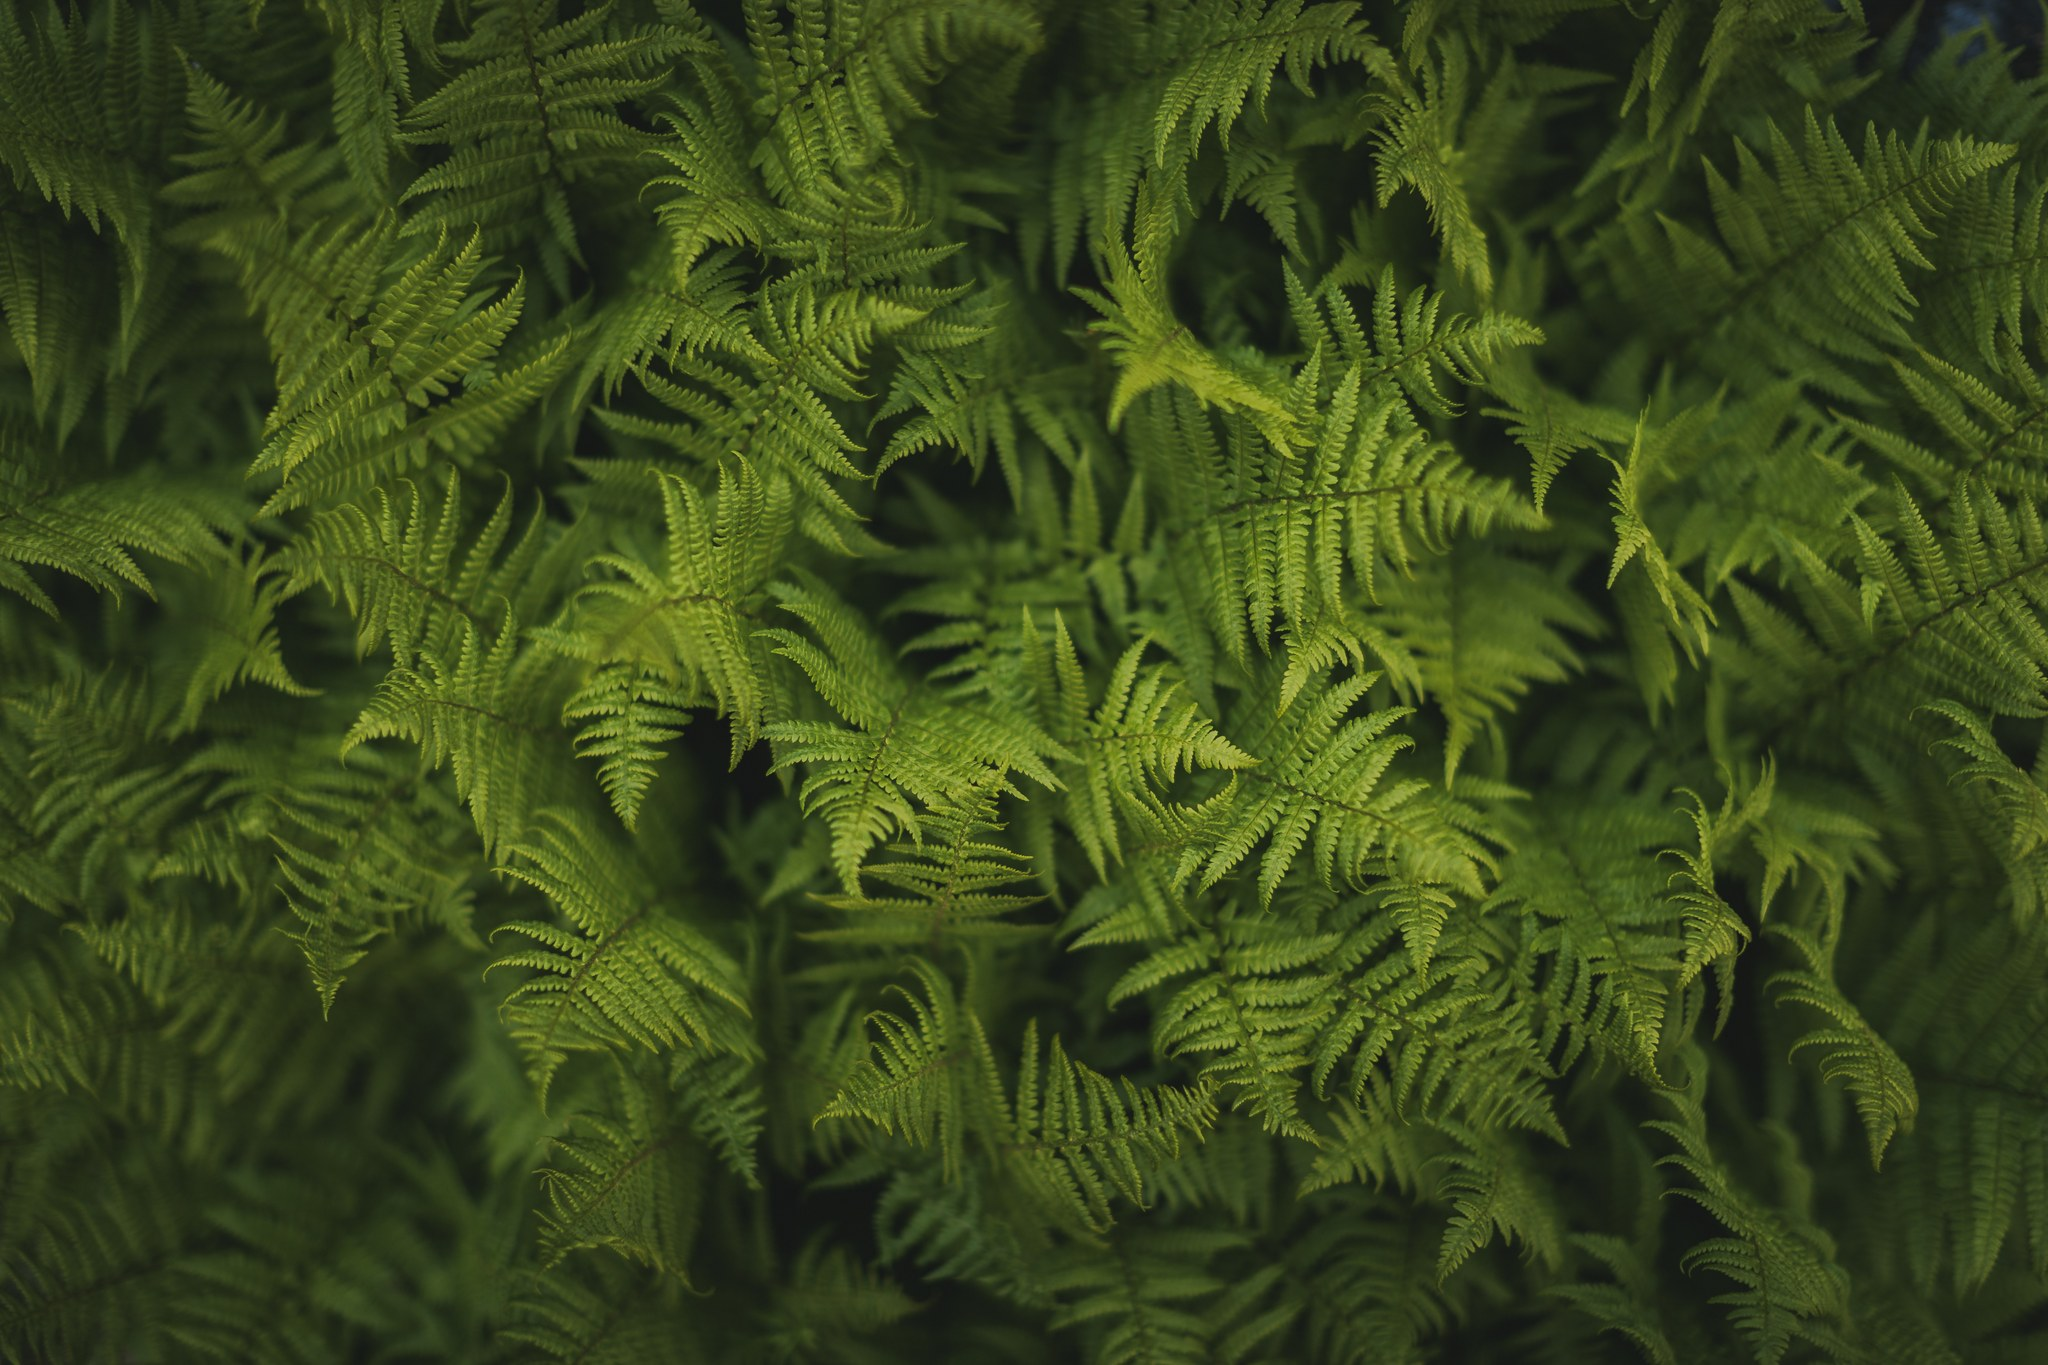
\includegraphics[
                                 width=\paperwidth,
                                 height=\paperheight]{logos/background_figure}
            };
        \end{tikzpicture}
        \begin{tikzpicture}[remember picture,overlay]
            \node[at=(current page.center)] {
                
\includegraphics[keepaspectratio,
                                 width=0.65\paperwidth,
                                 height=\paperheight]{logos/LUT-LOGO-WHITE-PNG}
            };
        \end{tikzpicture}
     \end{frame}
}

\end{document}
